\documentclass{article}


\usepackage{arxiv}

\usepackage[utf8]{inputenc} % allow utf-8 input
\usepackage[T1]{fontenc}    % use 8-bit T1 fonts
\usepackage{hyperref}       % hyperlinks
\usepackage{url}            % simple URL typesetting
\usepackage{booktabs}       % professional-quality tables
\usepackage{amsfonts}       % blackboard math symbols
\usepackage{amsmath}        % math environments (bmatrix, etc.)
\usepackage{nicefrac}       % compact symbols for 1/2, etc.
\usepackage{microtype}      % microtypography
\usepackage{lipsum}
\usepackage{graphicx}
\usepackage{tikz}
\usetikzlibrary{shapes.geometric, arrows.meta, positioning, fit, backgrounds, calc}
\graphicspath{ {./images/} }


\title{Design and Implementatison of a Monocular Measurement System on Android using Dynamic Camera Intrinsics}


\author{
 Trung Duc Bui \\
  School of Coumputing and Information\\
  University of Pittsburgh\\
  Pittsburgh, PA 15213 \\
  \texttt{trungbuiducbuiduc@gmail.com}
}

\begin{document}
\maketitle
\begin{abstract}
   Estimating real-world object dimensions from smartphone images is a fundamental problem in computer vision, with applications in e-commerce, logistics, and interior design. Commercial solutions typically rely on augmented reality (AR) frameworks such as ARCore or ARKit, which provide metric scale through SLAM-based 3D reconstruction. However, these frameworks act as ``black boxes'' that obscure the underlying geometric principles, impose operational constraints, and---critically---are not available on all devices, as ARCore certification covers only a subset of Android smartphones. This paper presents the design and implementation of a \textit{traditional, AR-free measurement pipeline} for Android that operates independently of proprietary AR SDKs, enabling metric measurement on any device with Camera2 API support. The proposed system implements a \textit{Dynamic Intrinsics} mechanism, recalculating the camera matrix $K$ per-frame based on \texttt{SCALER\_CROP\_REGION} metadata to maintain accuracy across continuous digital zoom levels. By fusing optical data with IMU-derived orientation, the system supports classical measurement models including ground-plane homography, planar object rectification, and single-view metrology. The application features a dual-mode design: a simplified \textit{User Mode} for practical measurement tasks, and a dedicated \textit{Researcher Mode} that exposes internal parameters and enables experimental analysis. To validate the proposed approach, we conduct systematic experiments using two devices: a non-ARCore device (Xiaomi Poco X6 Pro) for the traditional pipeline and an ARCore-certified device (Google Pixel 7 Pro) for baseline comparison. Results demonstrate that classical computer vision techniques, when properly controlled for intrinsic parameter variations, can achieve accuracy comparable to AR-based approaches while offering superior transparency, interpretability, and broader device compatibility.
\end{abstract}


% keywords can be removed
\keywords{Single-View Metrology \and Dynamic Camera Intrinsics \and Android Camera2 API \and Digital Zoom Compensation \and Pinhole Camera Model \and Ground-Plane Homography \and ARCore Comparison \and Mobile Measurement}


\section{Introduction}

Estimating real-world object dimensions from images captured by consumer smartphones is a fundamental problem in computer vision, with practical applications spanning e-commerce (product sizing), logistics (package dimensioning), interior design (room measurement), and augmented reality. Over the past decade, mobile devices have witnessed remarkable advances in optical hardware, equipping modern smartphones with high-resolution sensors, optical image stabilization (OIS), and low-level hardware access via APIs such as Android's Camera2. While this evolution positions smartphones as potential precision instruments for metrology, realizing a mathematically transparent measurement tool remains a significant challenge.

Commercial measurement solutions typically rely on augmented reality (AR) frameworks such as ARCore or ARKit, which provide metric scale through visual-inertial odometry (VIO) and simultaneous localization and mapping (SLAM). While these approaches can achieve practical accuracy, they exhibit fundamental limitations: they act as ``black boxes'' that obscure the underlying geometric principles, impose operational constraints (requiring camera motion for initialization, texture-rich environments), and---importantly---are not available on all Android devices. As of 2024, ARCore supports only a curated list of certified devices, leaving many capable smartphones without access to AR-based measurement. For researchers and learners seeking to understand, validate, or modify the measurement models, such opacity and limited availability represent significant barriers.

A particularly underexplored challenge within this domain is the \textit{dynamic nature of camera intrinsics during digital zoom operations}. Unlike optical zoom which physically adjusts lens elements, digital zoom fundamentally alters the effective camera matrix through sensor cropping and resampling. The intrinsic parameters---focal length and principal point---change with each zoom level, yet standard measurement applications often assume a fixed camera matrix, leading to systematic errors that compound at higher magnification. This problem is exacerbated by the fact that few existing systems leverage the rich per-frame metadata available through the Camera2 API, particularly \texttt{SCALER\_CROP\_REGION}.

To address these challenges, we present a configurable monocular measurement system for Android that operates independently of third-party AR frameworks. The proposed system targets two distinct audiences:
\begin{enumerate}
   \item \textbf{End-users}, who require a simple, accessible tool to measure objects quickly and accurately; and
   \item \textbf{Researchers and learners}, who seek to understand, inspect, and experiment with the underlying camera model and geometric assumptions.
\end{enumerate}

The system implements a \textit{Dynamic Intrinsics} mechanism that continuously recalculates the camera matrix $K$ based on real-time \texttt{SCALER\_CROP\_REGION} metadata, maintaining measurement accuracy across continuous zoom levels. By fusing optical data with IMU-derived orientation, the system supports classical measurement models---including ground-plane homography, planar object rectification, and single-view metrology---through a transparent, fully controllable pipeline.

Uniquely, the application features a dual-mode design: a simplified \textit{User Mode} for practical measurement tasks, and a dedicated \textit{Researcher Mode} that exposes all internal parameters, supports toggling of processing options (undistortion, edge snapping, rectification, multi-frame averaging), and enables export of detailed logs for analysis. To validate the proposed approach against the state of practice, we conduct systematic experiments using two devices: a non-ARCore-certified device (Xiaomi Poco X6 Pro) running the traditional pipeline, and an ARCore-certified device (Google Pixel 7 Pro) for baseline comparison. This setup directly addresses the practical question: \textit{can a traditional, Camera2-based pipeline achieve comparable accuracy to ARCore on devices where AR frameworks are unavailable?}

The main contributions of this work are:
\begin{enumerate}
   \item A \textbf{camera-model-driven measurement pipeline} for Android that uses Camera2 metadata (intrinsic calibration, active array size, dynamic crop region) to reconstruct a per-frame intrinsic matrix $K_{out}$, maintaining accuracy across continuous digital zoom levels.

   \item A \textbf{dual-mode application design} with a user-friendly interface for end-users and a dedicated Researcher Mode that exposes internal parameters, processing steps, and experimental controls for educational and research purposes.

   \item A \textbf{systematic experimental evaluation} comparing the traditional pipeline with an ARCore-based baseline using two devices (non-ARCore vs. ARCore-certified), demonstrating that classical techniques can achieve comparable accuracy even on devices where AR frameworks are unavailable.
\end{enumerate}

The remainder of this paper is organized as follows. Section~\ref{sec:literature} reviews related work on camera calibration, single-view metrology, and existing measurement approaches. Section~\ref{sec:system} describes the proposed system architecture and measurement modules. Section~\ref{sec:experiment} presents the experimental setup and methodology. Section~\ref{sec:results} reports results and discussion. Section~\ref{sec:conclusion} concludes the paper, and Section~\ref{sec:future} outlines directions for future work.

\section{Literature Review}
\label{sec:literature}

This section establishes the theoretical foundations of the proposed system, covering the geometric modeling of cameras, the specific challenges of digital image formation on mobile devices, and existing techniques for extracting metric dimensions from 2D images.

\subsection{Pinhole Camera Model and Calibration}

\subsubsection{The Pinhole Model}

The pinhole camera model serves as the fundamental geometric abstraction for image formation in computer vision~\cite{hartley2003multiple}. This idealized model assumes that all light rays pass through a single point (the optical center) before striking the image plane. Under this model, a 3D world point $\mathbf{X}_w = (X, Y, Z)^T$ is projected onto the 2D image plane at pixel coordinates $(u, v)$ through a linear transformation in homogeneous coordinates:

\begin{equation}
   s \begin{bmatrix} u \\ v \\ 1 \end{bmatrix} = K [R \mid t] \begin{bmatrix} X \\ Y \\ Z \\ 1 \end{bmatrix}
   \label{eq:pinhole}
\end{equation}

where $s$ is an arbitrary scale factor arising from the use of homogeneous coordinates. The $3 \times 4$ projection matrix $P = K[R \mid t]$ decomposes into two components: the \textit{extrinsic parameters} $[R \mid t]$ describing the camera's pose (rotation $R \in SO(3)$ and translation $t \in \mathbb{R}^3$) in world coordinates, and the \textit{intrinsic matrix} $K$ encoding the internal camera geometry:

\begin{equation}
   K = \begin{bmatrix}
      f_x & s   & c_x \\
      0   & f_y & c_y \\
      0   & 0   & 1
   \end{bmatrix}
   \label{eq:intrinsic}
\end{equation}

Here, $f_x$ and $f_y$ represent the focal length expressed in pixel units along the horizontal and vertical axes respectively, $(c_x, c_y)$ denotes the principal point (the intersection of the optical axis with the image plane), and $s$ is the skew coefficient (typically zero for modern sensors with rectangular pixels).

% ============ FIGURE PLACEHOLDER ============
% TODO: Add Figure - Pinhole camera geometry diagram
% Content: 3D illustration showing world coordinate system, camera coordinate system,
% optical center, image plane, and the projection of a 3D point onto the image.
% Caption: "The pinhole camera model: a 3D point X is projected through the optical center O onto the image plane at pixel coordinates (u,v)."
% \begin{figure}[h]
%     \centering
%     \includegraphics[width=0.8\textwidth]{figures/pinhole_model.pdf}
%     \caption{The pinhole camera model geometry showing the projection of a 3D world point onto the 2D image plane.}
%     \label{fig:pinhole_model}
% \end{figure}
% =============================================

\subsubsection{Lens Distortion}

Real camera lenses deviate from the ideal pinhole model by introducing geometric distortions. The two primary types are:

\textbf{Radial distortion} causes straight lines to appear curved, particularly near the image periphery. It is modeled as a polynomial function of the distance $r$ from the principal point:
\begin{equation}
   \begin{aligned}
      x_{distorted} & = x(1 + k_1 r^2 + k_2 r^4 + k_3 r^6) \\
      y_{distorted} & = y(1 + k_1 r^2 + k_2 r^4 + k_3 r^6)
   \end{aligned}
   \label{eq:radial_distortion}
\end{equation}
where $(x, y)$ are normalized image coordinates and $k_1, k_2, k_3$ are the radial distortion coefficients. Positive coefficients produce barrel distortion (lines curve outward), while negative coefficients produce pincushion distortion (lines curve inward).

\textbf{Tangential distortion} arises from imperfect alignment between the lens elements and the image sensor, causing asymmetric displacement:
\begin{equation}
   \begin{aligned}
      x_{distorted} & = x + [2p_1 xy + p_2(r^2 + 2x^2)] \\
      y_{distorted} & = y + [p_1(r^2 + 2y^2) + 2p_2 xy]
   \end{aligned}
   \label{eq:tangential_distortion}
\end{equation}
where $p_1, p_2$ are the tangential distortion coefficients.

For accurate metric measurement, these distortions must be corrected through an \textit{undistortion} process that maps observed pixel coordinates to their ideal positions.

% ============ FIGURE PLACEHOLDER ============
% TODO: Add Figure - Lens distortion visualization
% Content: Side-by-side comparison showing (a) barrel distortion, (b) pincushion distortion,
% (c) original grid pattern, (d) undistorted result
% Caption: "Types of lens distortion: (a) barrel distortion (k1 > 0), (b) pincushion distortion (k1 < 0), and (c) the effect of undistortion on a checkerboard pattern."
% \begin{figure}[h]
%     \centering
%     \includegraphics[width=0.9\textwidth]{figures/distortion_types.pdf}
%     \caption{Visualization of radial lens distortion types and the undistortion correction process.}
%     \label{fig:distortion}
% \end{figure}
% =============================================

\subsubsection{Camera Calibration Techniques}

Camera calibration is the process of estimating the intrinsic parameters $K$ and distortion coefficients from images of known patterns. Zhang's flexible calibration method~\cite{zhang2000flexible} revolutionized this process by requiring only a planar calibration target (typically a checkerboard) captured at multiple orientations.

The procedure involves:
\begin{enumerate}
   \item \textbf{Pattern detection}: Locating grid corners in each calibration image using algorithms such as \texttt{findChessboardCorners}.
   \item \textbf{Subpixel refinement}: Improving corner localization accuracy to 0.1 pixels or better using gradient-based methods (\texttt{cornerSubPix}).
   \item \textbf{Homography estimation}: Computing the $3 \times 3$ homography $H_i$ mapping pattern coordinates to image coordinates for each view.
   \item \textbf{Intrinsic extraction}: Exploiting constraints on the absolute conic to solve for $K$ from multiple homographies.
   \item \textbf{Extrinsic recovery}: Computing rotation and translation for each view given $K$.
   \item \textbf{Nonlinear refinement}: Minimizing the total reprojection error over all views using Levenberg-Marquardt optimization.
\end{enumerate}

The reprojection error---the RMS distance between observed corners and their predicted positions---serves as a quality metric; values below 0.5 pixels indicate excellent calibration. More recent calibration targets such as ChArUco boards~\cite{garrido2014charuco} combine the corner accuracy of checkerboards with the robustness of ArUco fiducial markers, enabling reliable detection even when the pattern is partially occluded or captured at extreme angles.

% ============ FIGURE PLACEHOLDER ============
% TODO: Add Figure - Calibration process
% Content: (a) Example checkerboard images at various orientations, (b) detected corners overlay,
% (c) reprojection error visualization
% Caption: "Camera calibration using Zhang's method: (a) checkerboard captured at multiple orientations, (b) detected and refined corner positions, (c) reprojection error distribution."
% \begin{figure}[h]
%     \centering
%     \includegraphics[width=\textwidth]{figures/calibration_process.pdf}
%     \caption{Zhang's camera calibration method using planar checkerboard patterns.}
%     \label{fig:calibration}
% \end{figure}
% =============================================

\subsection{Single-View Metrology}

Single-view metrology addresses the recovery of metric information from a single 2D image using projective geometry constraints~\cite{criminisi2000single}. This is fundamentally an ill-posed problem since depth information is lost during projection; however, additional constraints---such as known geometry, scene planarity, or reference dimensions---can make metric reconstruction tractable.

\subsubsection{Homography and Ground-Plane Measurement}

When measuring objects that lie on a known plane (e.g., the ground or a table surface), the image-to-world mapping simplifies considerably. For a plane at $Z = 0$ in world coordinates, the projection equation reduces to a $3 \times 3$ homography $H$:

\begin{equation}
   s \begin{bmatrix} u \\ v \\ 1 \end{bmatrix} = H \begin{bmatrix} X \\ Y \\ 1 \end{bmatrix}, \quad H = K [r_1 \mid r_2 \mid t]
   \label{eq:homography}
\end{equation}

where $r_1, r_2$ are the first two columns of the rotation matrix $R$ and $t$ is the translation. Given knowledge of the camera's intrinsic matrix $K$, height $h$ above the ground plane, and orientation from an inertial measurement unit (IMU), the homography $H$ can be computed analytically. The inverse homography $H^{-1}$ then maps any image point $(u, v)$ to ground coordinates $(X, Y)$, enabling direct distance computation:

\begin{equation}
   d = \sqrt{(X_A - X_B)^2 + (Y_A - Y_B)^2}
   \label{eq:ground_distance}
\end{equation}

This approach is particularly effective for measuring horizontal distances on floors, tables, or other flat surfaces when the camera pose is known.

% ============ FIGURE PLACEHOLDER ============
% TODO: Add Figure - Ground-plane homography
% Content: Diagram showing camera above ground plane, coordinate systems, homography mapping,
% and measurement between two points A and B on the ground
% Caption: "Ground-plane homography: the camera at height h above the ground enables mapping of image points to world coordinates for distance measurement."
% \begin{figure}[h]
%     \centering
%     \includegraphics[width=0.85\textwidth]{figures/ground_plane_homography.pdf}
%     \caption{Ground-plane measurement using homography derived from camera height and orientation.}
%     \label{fig:ground_homography}
% \end{figure}
% =============================================

\subsubsection{Planar Object Rectification}

For planar objects not aligned with the ground (e.g., a wall-mounted poster, a box face, or a sheet of paper), perspective rectification enables measurement. Given four corner points of a rectangular object in the image, a homography $H_{rect}$ can be computed to warp the object to a fronto-parallel (orthogonal) view:

\begin{equation}
   H_{rect}: (u_i, v_i) \rightarrow (x'_i, y'_i), \quad i = 1, 2, 3, 4
\end{equation}

In the rectified image, the object appears as a rectangle without perspective distortion. If the approximate distance $Z$ from the camera to the object plane is known (e.g., from autofocus metadata or user input), the pixel-to-metric scale can be derived from the pinhole model:

\begin{equation}
   L_{real} = \frac{L_{pixels} \cdot Z}{f}
   \label{eq:pinhole_scale}
\end{equation}

where $f$ is the focal length and $L_{pixels}$ is the measured length in the rectified image.

\subsubsection{Vanishing Points and Cross-Ratio}

For scenes with strong perspective effects---such as tall buildings, corridors, or streets---vanishing point analysis provides powerful geometric constraints~\cite{cipolla1999camera}. Parallel lines in 3D space converge to a vanishing point (VP) in the image; three mutually orthogonal vanishing points (corresponding to the X, Y, and Z world axes) fully constrain the camera's orientation.

The cross-ratio, a projective invariant preserved under perspective projection, enables height estimation from a single image. Given a vertical structure with its base at ground level, if the camera height $h_{cam}$ is known and the horizon line (connecting horizontal vanishing points) is identified, the ratio of image distances can be used to compute the unknown object height $h_{obj}$:

\begin{equation}
   h_{obj} = h_{cam} \cdot \frac{d(base, top)}{d(base, horizon)}
   \label{eq:cross_ratio}
\end{equation}

where $d(\cdot, \cdot)$ denotes the signed distance along the vertical image direction.

% ============ FIGURE PLACEHOLDER ============
% TODO: Add Figure - Vanishing points and height estimation
% Content: (a) Image with detected lines and computed vanishing points,
% (b) Horizon line and vertical measurement diagram,
% (c) Cross-ratio geometry for height estimation
% Caption: "Single-view metrology using vanishing points: (a) vanishing point detection from parallel lines, (b) horizon line determination, (c) height estimation using cross-ratio."
% \begin{figure}[h]
%     \centering
%     \includegraphics[width=\textwidth]{figures/vanishing_points.pdf}
%     \caption{Vanishing point detection and cross-ratio based height estimation.}
%     \label{fig:vanishing_points}
% \end{figure}
% =============================================

\subsection{Smartphone Camera Systems and the Android Camera2 API}

Modern smartphones integrate sophisticated camera systems that present both opportunities and challenges for metrology applications. This section examines the hardware characteristics and software interfaces relevant to measurement accuracy.

\subsubsection{Smartphone Camera Hardware}

Contemporary smartphone cameras feature:
\begin{itemize}
   \item \textbf{High-resolution sensors}: Typical resolutions of 12--200 megapixels, with pixel sizes ranging from 0.7 to 1.8 $\mu m$.
   \item \textbf{Multi-camera arrays}: Wide, ultra-wide, and telephoto lenses with different intrinsic parameters.
   \item \textbf{Optical Image Stabilization (OIS)}: Physical lens displacement to compensate for hand shake, which can affect the effective optical axis.
   \item \textbf{Autofocus systems}: Phase-detection or contrast-detection AF providing focus distance metadata.
   \item \textbf{Inertial Measurement Units (IMU)}: Accelerometers and gyroscopes providing device orientation.
\end{itemize}

Unlike professional cameras with fixed, well-characterized lenses, smartphone cameras exhibit significant variation in intrinsic parameters across devices and may not provide accurate factory calibration.

\subsubsection{The Camera2 API and Intrinsic Metadata}

The Android Camera2 API~\cite{android_camera2} provides low-level access to camera hardware, exposing metadata critical for geometric applications. Key fields include:

\begin{itemize}
   \item \texttt{LENS\_INTRINSIC\_CALIBRATION}: A 5-element array $(f_x, f_y, c_x, c_y, s)$ providing manufacturer-calibrated intrinsic parameters in pixels, defined relative to the sensor's active array coordinate system.

   \item \texttt{SENSOR\_INFO\_ACTIVE\_ARRAY\_SIZE}: The dimensions $(W_s, H_s)$ of the sensor's light-sensitive area in pixels.

   \item \texttt{SENSOR\_INFO\_PHYSICAL\_SIZE}: The physical dimensions of the active array in millimeters, enabling conversion between pixel and metric focal lengths.

   \item \texttt{LENS\_RADIAL\_DISTORTION}: Radial distortion coefficients (when available; many devices report this as unavailable).

   \item \texttt{LENS\_POSE\_ROTATION} and \texttt{LENS\_POSE\_TRANSLATION}: The pose of the camera relative to the device's IMU coordinate frame.
\end{itemize}

The availability and accuracy of these fields vary significantly across devices. For example, our target device (Xiaomi Poco X6 Pro) provides \texttt{LENS\_INTRINSIC\_CALIBRATION} but reports \texttt{LENS\_RADIAL\_DISTORTION} as unavailable.

\subsubsection{Digital Zoom and the Dynamic Crop Region}

A critical challenge for measurement applications is handling digital zoom. Unlike optical zoom, which physically adjusts lens elements and changes the optical focal length, digital zoom operates entirely in the image processing pipeline by:

\begin{enumerate}
   \item Cropping a subregion of the sensor (the ``crop region'')
   \item Scaling the cropped region to the output resolution through interpolation
\end{enumerate}

The \texttt{SCALER\_CROP\_REGION} field in \texttt{CaptureResult} specifies the active crop rectangle $(x_0, y_0, w_c, h_c)$ for each captured frame. This dynamic cropping fundamentally alters the effective intrinsic parameters:

\begin{itemize}
   \item The \textbf{principal point shifts} from $(c_x, c_y)$ to $(c_x - x_0, c_y - y_0)$ in crop coordinates.
   \item The \textbf{effective focal length scales} by the ratio $s_x = W_{out}/w_c$ (horizontal) and $s_y = H_{out}/h_c$ (vertical).
\end{itemize}

The per-frame intrinsic matrix for the output image becomes:

\begin{equation}
   K_{out} = \begin{bmatrix}
      f_x \cdot s_x & 0             & (c_x - x_0) \cdot s_x \\
      0             & f_y \cdot s_y & (c_y - y_0) \cdot s_y \\
      0             & 0             & 1
   \end{bmatrix}
   \label{eq:dynamic_intrinsics}
\end{equation}

Failure to account for these dynamic changes leads to systematic measurement errors that grow with zoom level---a problem largely overlooked by existing measurement applications.

% ============ FIGURE PLACEHOLDER ============
% TODO: Add Figure - Digital zoom and crop region
% Content: (a) Full sensor active array with intrinsic coordinate system,
% (b) Crop region at different zoom levels (1x, 2x, 3x),
% (c) Diagram showing how principal point and focal length transform
% Caption: "Dynamic intrinsics under digital zoom: (a) the full sensor active array, (b) crop regions at increasing zoom levels, (c) the transformation of intrinsic parameters."
% \begin{figure}[h]
%     \centering
%     \includegraphics[width=\textwidth]{figures/dynamic_intrinsics.pdf}
%     \caption{Digital zoom alters effective intrinsic parameters through sensor cropping and scaling.}
%     \label{fig:dynamic_intrinsics}
% \end{figure}
% =============================================

\subsection{Existing Measurement Approaches}

This section surveys existing approaches to smartphone-based measurement, categorizing them into AR-based and traditional methods.

\subsubsection{AR-Based Measurement Systems}

Commercial measurement applications such as Google's Measure app (using ARCore) and Apple's Measure app (using ARKit) leverage augmented reality frameworks to perform 3D reconstruction in real-time~\cite{arcore_overview}. These systems employ:

\begin{itemize}
   \item \textbf{Visual-Inertial Odometry (VIO)}: Fusing camera images with IMU data to track device motion with centimeter-level accuracy.
   \item \textbf{Simultaneous Localization and Mapping (SLAM)}: Building a sparse 3D map of the environment while simultaneously localizing the camera within it.
   \item \textbf{Plane Detection}: Identifying horizontal and vertical surfaces using geometric analysis of tracked feature points.
   \item \textbf{Depth Estimation}: On supported devices, utilizing time-of-flight (ToF) sensors or stereo cameras to obtain dense depth maps.
\end{itemize}

Users place virtual anchors on detected surfaces and the system computes Euclidean distances in metric world coordinates. Reported accuracies of 1--3\% for objects within 3 meters are common under favorable conditions~\cite{vogt2021ar_accuracy}.

However, AR-based approaches exhibit several fundamental limitations:

\begin{enumerate}
   \item \textbf{Opacity and non-transparency}: The geometric internals are hidden within proprietary frameworks, providing no insight into how measurements are computed. Users cannot inspect, validate, or modify the underlying models.

   \item \textbf{Operational constraints}: SLAM initialization requires camera motion to establish a baseline; tracking can fail in featureless, textureless, or highly reflective environments. The requirement for motion is impractical for quick, single-shot measurements.

   \item \textbf{Computational overhead}: Continuous SLAM processing imposes significant battery and thermal constraints.

   \item \textbf{Device requirements}: ARCore and ARKit are not universally available; older or budget devices may lack certification, limiting accessibility.

   \item \textbf{Environmental dependencies}: Performance degrades in low-light conditions, with moving objects, or on surfaces lacking sufficient texture.
\end{enumerate}

For educational purposes---where understanding the connection between geometric theory (pinhole model, homography, projective invariants) and practical measurement is paramount---such opacity represents a significant barrier.

% ============ FIGURE PLACEHOLDER ============
% TODO: Add Figure - AR measurement comparison
% Content: Screenshots of (a) ARCore Measure app in action, (b) typical failure cases
% (featureless surface, reflective floor), (c) comparison table of AR vs traditional approaches
% Caption: "AR-based measurement: (a) Google Measure app interface, (b) failure on reflective surfaces, (c) comparison of AR and traditional approaches."
% \begin{figure}[h]
%     \centering
%     \includegraphics[width=0.9\textwidth]{figures/ar_comparison.pdf}
%     \caption{AR-based measurement applications and their operational limitations.}
%     \label{fig:ar_measurement}
% \end{figure}
% =============================================

\subsubsection{Traditional Image-Based Measurement}

Alternative approaches have explored purely image-based measurement on smartphones using classical computer vision techniques:

\begin{itemize}
   \item \textbf{Fixed calibration methods}: Performing offline camera calibration with checkerboard patterns and storing the intrinsic matrix for subsequent use. However, these approaches typically ignore the effects of digital zoom.

   \item \textbf{Reference object methods}: Placing a known-size object (credit card, coin, ruler) in the scene to establish pixel-to-metric scale. While simple, this adds friction to the measurement workflow.

   \item \textbf{IMU-assisted ground-plane estimation}: Using device accelerometers and gyroscopes to estimate camera orientation, combined with a user-provided camera height to construct ground-plane homographies~\cite{mulloni2010handheld}.

   \item \textbf{Vanishing point methods}: Detecting scene geometry from parallel lines to recover camera orientation and apply cross-ratio based measurement~\cite{criminisi2000single}.
\end{itemize}

While these methods are transparent and educational, many exhibit significant limitations in practice:

\begin{enumerate}
   \item \textbf{Static intrinsic assumption}: Most systems assume a fixed camera matrix $K$ and fail to update it when users employ digital zoom, leading to systematic errors.

   \item \textbf{Neglect of Camera2 metadata}: Few systems leverage the rich per-frame metadata available through Camera2, particularly \texttt{SCALER\_CROP\_REGION}.

   \item \textbf{Limited processing options}: Users cannot easily compare the effects of different processing choices (undistortion on/off, different measurement models).

   \item \textbf{Lack of experimental validation}: Rigorous comparison against AR baselines under controlled conditions is rarely provided.
\end{enumerate}

\subsection{Research Gap and Contributions}

The existing literature reveals two significant gaps that this work addresses:

\begin{enumerate}
   \item \textbf{Lack of transparent, educational measurement systems}: Current AR-based tools act as ``black boxes,'' concealing the connection between geometric theory and practical measurement. For learners and researchers seeking to understand, validate, or modify the underlying models, such opacity is a significant barrier. There is a need for a measurement system that exposes every step of the pipeline---from raw sensor data to final metric output---enabling rigorous educational and experimental use.

   \item \textbf{Limited handling of dynamic intrinsics under zoom}: Few systems leverage the rich Camera2 metadata---particularly \texttt{SCALER\_CROP\_REGION}---to maintain correct intrinsic parameters across continuous zoom levels. This oversight results in zoom-dependent errors that compound at higher magnification. No prior work has systematically validated the dynamic intrinsics approach against both ground truth and AR baselines.
\end{enumerate}

Table~\ref{tab:related_work} summarizes the key characteristics of existing approaches compared to the proposed system.

% ============ TABLE PLACEHOLDER ============
% TODO: Add comparison table
\begin{table}[h]
   \centering
   \caption{Comparison of existing measurement approaches with the proposed system.}
   \label{tab:related_work}
   \begin{tabular}{lcccc}
      \toprule
      \textbf{Approach}        & \textbf{Transparency} & \textbf{Dynamic Zoom} & \textbf{No AR Required} & \textbf{Researcher Mode} \\
      \midrule
      ARCore/ARKit Apps        & Low                   & N/A (3D)              & No                      & No                       \\
      Fixed Calibration        & High                  & No                    & Yes                     & No                       \\
      Reference Object         & High                  & Partial               & Yes                     & No                       \\
      \textbf{Proposed System} & \textbf{High}         & \textbf{Yes}          & \textbf{Yes}            & \textbf{Yes}             \\
      \bottomrule
   \end{tabular}
\end{table}
% =============================================

This work addresses these gaps through the following contributions:

\begin{enumerate}
   \item A \textbf{Dynamic Intrinsics mechanism} that recalculates the camera matrix $K_{out}$ per-frame based on \texttt{SCALER\_CROP\_REGION} metadata, maintaining measurement accuracy across continuous zoom levels.

   \item A \textbf{transparent measurement pipeline} implementing classical techniques (ground-plane homography, planar rectification, single-view metrology) with full visibility into every processing step.

   \item A dedicated \textbf{Researcher Mode} that exposes all internal parameters, supports toggling of processing options (undistortion, edge snapping, rectification, multi-frame averaging), and enables export of detailed logs for analysis.

   \item \textbf{Systematic experimental comparison} against an ARCore baseline on the same device, providing empirical validation under controlled conditions across varying distances, zoom levels, and object types.
\end{enumerate}

\section{Proposed System}
\label{sec:system}

This section describes the architecture and implementation of the proposed measurement system. We present the overall system design, the dynamic intrinsics mechanism, the measurement modules, the image processing pipeline, and the dual-mode user interface.

\subsection{Overall Architecture}

The proposed application is implemented in Flutter with native Android modules for camera access (Camera2 API) and augmented reality (ARCore). The architecture follows a modular design that separates concerns and enables flexible configuration. Figure~\ref{fig:architecture} illustrates the system components.

% System Architecture Diagram using TikZ
\begin{figure}[htbp]
   \centering
   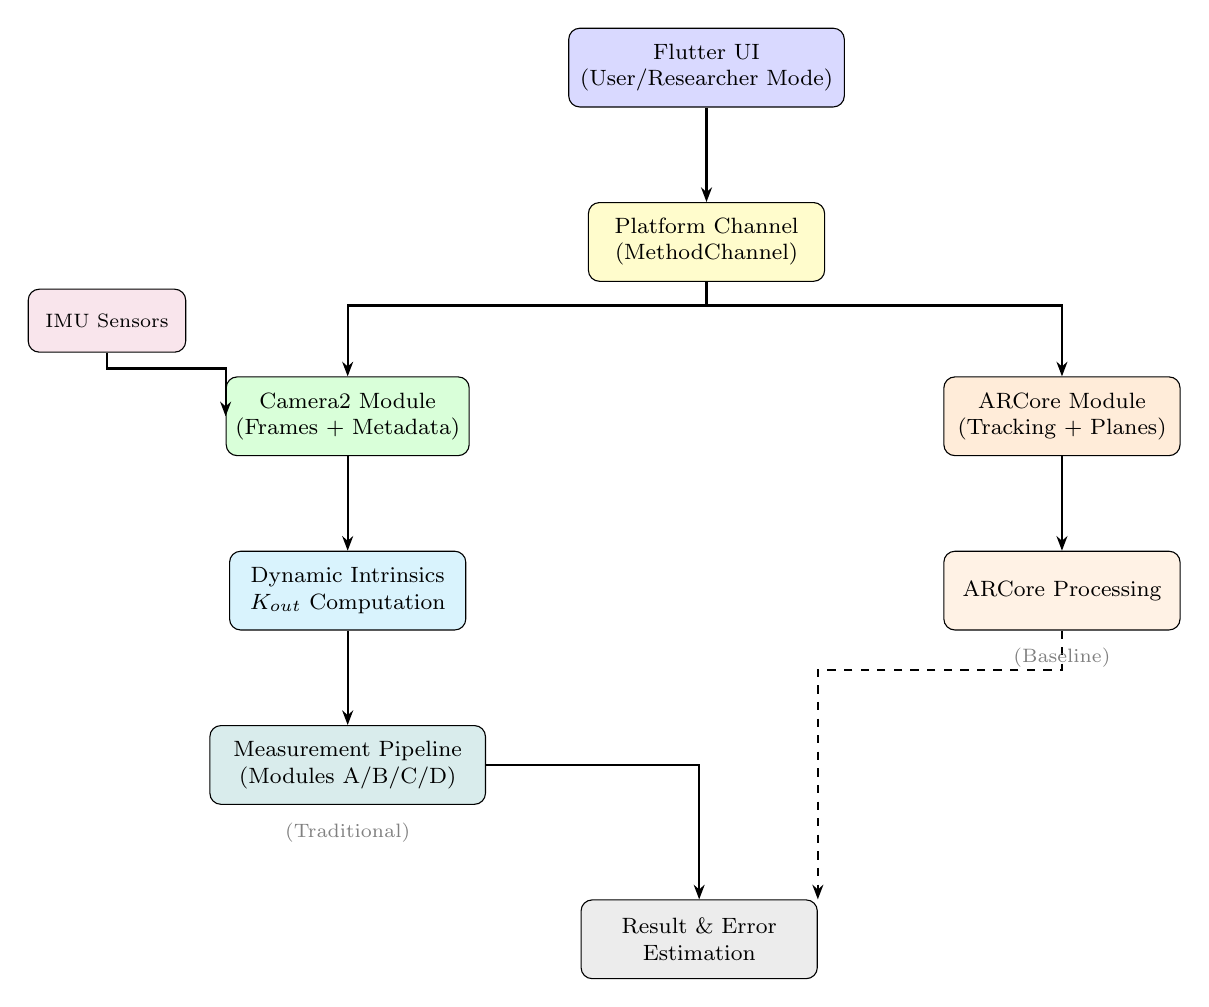
\begin{tikzpicture}[
      node distance=1.2cm and 2.5cm,
      box/.style={rectangle, draw, rounded corners, minimum width=3cm, minimum height=1cm, align=center, font=\footnotesize},
      bigbox/.style={rectangle, draw, rounded corners, minimum width=3.5cm, minimum height=1cm, align=center, font=\footnotesize},
      smallbox/.style={rectangle, draw, rounded corners, minimum width=2cm, minimum height=0.8cm, align=center, font=\scriptsize},
      arrow/.style={-{Stealth[scale=0.8]}, thick},
      dashedarrow/.style={-{Stealth[scale=0.8]}, thick, dashed}
      ]

      % Flutter UI Layer
      \node[bigbox, fill=blue!15] (ui) {Flutter UI\\(User/Researcher Mode)};

      % Platform Channel
      \node[box, below=1.2cm of ui, fill=yellow!20] (channel) {Platform Channel\\(MethodChannel)};

      % Native Modules - spread wider
      \node[box, below left=1.2cm and 1.5cm of channel, fill=green!15] (camera2) {Camera2 Module\\(Frames + Metadata)};
      \node[box, below right=1.2cm and 1.5cm of channel, fill=orange!15] (arcore) {ARCore Module\\(Tracking + Planes)};

      % IMU - positioned above-left of camera2
      \node[smallbox, above left=0.3cm and 0.5cm of camera2, fill=purple!10] (imu) {IMU Sensors};

      % Processing Layer
      \node[box, below=1.2cm of camera2, fill=cyan!15] (dynK) {Dynamic Intrinsics\\$K_{out}$ Computation};
      \node[box, below=1.2cm of arcore, fill=orange!10] (arprocess) {ARCore Processing};

      % Measurement Pipeline - centered below dynK
      \node[bigbox, below=1.2cm of dynK, fill=teal!15] (pipeline) {Measurement Pipeline\\(Modules A/B/C/D)};

      % Result - centered between pipeline and arprocess
      \node[box, below right=1.2cm and 0cm of pipeline, xshift=1.2cm, fill=gray!15] (result) {Result \& Error\\Estimation};

      % Arrows - main flow
      \draw[arrow] (ui) -- (channel);
      \draw[arrow] (channel.south) -- ++(0,-0.3) -| (camera2.north);
      \draw[arrow] (channel.south) -- ++(0,-0.3) -| (arcore.north);
      \draw[arrow] (imu.south) -- ++(0,-0.2) -| (camera2.west);
      \draw[arrow] (camera2) -- (dynK);
      \draw[arrow] (arcore) -- (arprocess);
      \draw[arrow] (dynK) -- (pipeline);
      \draw[arrow] (pipeline.east) -| (result.north);
      \draw[dashedarrow] (arprocess.south) -- ++(0,-0.5) -| (result.north east);

      % Labels - positioned clearly
      \node[below=0.1cm of arprocess, font=\scriptsize, text=gray] {(Baseline)};
      \node[below=0.1cm of pipeline, font=\scriptsize, text=gray] {(Traditional)};

   \end{tikzpicture}
   \caption{Overall system architecture showing the Flutter application layer, native Android modules (Camera2 and ARCore), and the measurement pipeline. Solid arrows indicate the traditional flow (main contribution); dashed arrows indicate the ARCore baseline flow.}
   \label{fig:architecture}
\end{figure}

The system supports two parallel measurement flows:

\begin{enumerate}
   \item \textbf{Traditional Flow (main contribution)}: Uses Camera2 to capture frames and per-frame metadata, computes dynamic intrinsics, and applies classical geometric measurement techniques.

   \item \textbf{ARCore Flow (baseline)}: Uses ARCore for visual-inertial tracking and plane detection, enabling 3D anchor placement and direct metric distance computation for comparison purposes.
\end{enumerate}

\subsubsection{Data Acquisition Layer}

The data acquisition layer interfaces with the device hardware through the Android Camera2 API and sensor framework:

\begin{itemize}
   \item \textbf{Camera2 Session}: Captures frames in YUV or JPEG format at configurable resolutions. Each frame is accompanied by a \texttt{CaptureResult} containing real-time metadata.

   \item \textbf{Camera Characteristics}: Provides static device information including \texttt{LENS\_INTRINSIC\_CALIBRATION}, \texttt{SENSOR\_INFO\_ACTIVE\_ARRAY\_SIZE}, and \texttt{SENSOR\_INFO\_PHYSICAL\_SIZE}.

   \item \textbf{IMU Sensors}: Accelerometer and gyroscope data are fused using a complementary filter to provide device orientation (roll, pitch, yaw) relative to gravity.

   \item \textbf{Platform Channel}: A Flutter MethodChannel bridges the native Android code and the Dart application layer, passing frame data, metadata, and measurement results.
\end{itemize}

\subsection{Camera Model and Dynamic Intrinsics}

The core innovation of this system is the \textit{Dynamic Intrinsics} mechanism that maintains correct camera parameters across continuous digital zoom levels.

\subsubsection{Intrinsic Parameter Sources}

The system supports two sources of intrinsic parameters:

\begin{enumerate}
   \item \textbf{Device Intrinsics (Default)}: Uses the manufacturer-provided \texttt{LENS\_INTRINSIC\_CALIBRATION} from Camera2, which provides $(f_x, f_y, c_x, c_y, s)$ in the sensor's active array coordinate system. Distortion coefficients from \texttt{LENS\_RADIAL\_DISTORTION} are used when available.

   \item \textbf{Custom Calibration (Researcher Mode)}: Users can perform offline calibration using a ChArUco board, capturing 20--40 images at various orientations. The calibration procedure yields custom $K_{self}$ and distortion coefficients, stored as JSON for later use. This enables comparison between device-provided and self-calibrated parameters.
\end{enumerate}

\subsubsection{Dynamic Intrinsics Computation}

When digital zoom is applied, the camera crops a subregion of the sensor and scales it to the output resolution. The \texttt{SCALER\_CROP\_REGION} field in each \texttt{CaptureResult} specifies the active crop rectangle. The dynamic intrinsics are computed as follows:

Let $(W_s, H_s)$ denote the sensor's active array dimensions, $(f_{x,s}, f_{y,s}, c_{x,s}, c_{y,s})$ the device intrinsics in active array coordinates, and $(x_0, y_0, w_c, h_c)$ the current crop region. For output image dimensions $(W_{out}, H_{out})$:

\textbf{Step 1: Transform to crop coordinates.}
\begin{equation}
   c_{x,c} = c_{x,s} - x_0, \quad c_{y,c} = c_{y,s} - y_0
\end{equation}

\textbf{Step 2: Compute scale factors.}
\begin{equation}
   s_x = \frac{W_{out}}{w_c}, \quad s_y = \frac{H_{out}}{h_c}
\end{equation}

\textbf{Step 3: Compute output intrinsics.}
\begin{equation}
   f_{x,out} = f_{x,s} \cdot s_x, \quad f_{y,out} = f_{y,s} \cdot s_y
\end{equation}
\begin{equation}
   c_{x,out} = c_{x,c} \cdot s_x, \quad c_{y,out} = c_{y,c} \cdot s_y
\end{equation}

The resulting per-frame intrinsic matrix is:
\begin{equation}
   K_{out} = \begin{bmatrix}
      f_{x,out} & 0         & c_{x,out} \\
      0         & f_{y,out} & c_{y,out} \\
      0         & 0         & 1
   \end{bmatrix}
   \label{eq:kout_final}
\end{equation}

This matrix is recomputed for every captured frame, ensuring that measurements remain accurate regardless of zoom level.

% ============ FIGURE PLACEHOLDER ============
% TODO: Add Figure - Dynamic intrinsics computation
% Content: Diagram showing (a) full active array with intrinsic coordinates,
% (b) crop region at zoom 2x, (c) output image with transformed intrinsics
% \begin{figure}[h]
%     \centering
%     \includegraphics[width=\textwidth]{figures/dynamic_intrinsics_computation.pdf}
%     \caption{Dynamic intrinsics computation: the crop region transforms the intrinsic parameters from sensor coordinates to output image coordinates.}
%     \label{fig:dynamic_intrinsics_comp}
% \end{figure}
% =============================================

\subsection{Measurement Modules}

The system implements four measurement modules, each targeting different scene configurations and geometric assumptions. Figure~\ref{fig:pipeline_flowchart} illustrates the complete measurement pipeline from input to output.

\subsubsection{Module A: Ground-Plane Measurement}

This module measures distances between points lying on a horizontal ground plane (floor, table). The approach constructs a homography between the image and the ground plane using:

\begin{itemize}
   \item Camera height $h$ above the ground (user-provided or measured)
   \item Camera orientation $R$ from IMU sensors
   \item Intrinsic matrix $K_{out}$
\end{itemize}

The ground plane is defined as $Z = 0$ in world coordinates with normal $\mathbf{n} = (0, 0, 1)^T$. The camera position is $\mathbf{t} = (0, 0, h)^T$. The homography from ground to image is:
\begin{equation}
   H = K_{out} [r_1 \mid r_2 \mid \mathbf{t}_{proj}]
\end{equation}
where $r_1, r_2$ are the first two columns of $R$.

To measure, the user selects two points $A(u_A, v_A)$ and $B(u_B, v_B)$ on the image. These are mapped to ground coordinates via:
\begin{equation}
   (X_A, Y_A) = H^{-1}(u_A, v_A), \quad (X_B, Y_B) = H^{-1}(u_B, v_B)
\end{equation}

The metric distance is:
\begin{equation}
   d = \sqrt{(X_A - X_B)^2 + (Y_A - Y_B)^2}
\end{equation}

% ============ FIGURE PLACEHOLDER ============
% TODO: Add Figure - Ground-plane measurement workflow
% Content: (a) User holding phone above ground, (b) image with selected points,
% (c) ground plane projection diagram
% \begin{figure}[h]
%     \centering
%     \includegraphics[width=0.9\textwidth]{figures/ground_plane_measurement.pdf}
%     \caption{Ground-plane measurement: (a) physical setup, (b) point selection on image, (c) geometric projection.}
%     \label{fig:ground_plane_module}
% \end{figure}
% =============================================

\subsubsection{Module B: Planar Object Measurement}

This module measures dimensions of planar objects (paper, screens, box faces) that may not be aligned with the ground. The workflow involves:

\begin{enumerate}
   \item \textbf{Corner Detection}: The user selects four corners of a rectangular object, or the system auto-detects them using Canny edge detection, Hough lines, contour approximation, and subpixel corner refinement.

   \item \textbf{Perspective Rectification}: A homography $H_{rect}$ warps the quadrilateral to a fronto-parallel rectangle:
         \begin{equation}
            H_{rect}: (u_i, v_i) \rightarrow (x'_i, y'_i), \quad i = 1, \ldots, 4
         \end{equation}

   \item \textbf{Scale Estimation}: The pixel-to-metric scale requires knowledge of the object-to-camera distance $Z$. This distance can be obtained from:
         \begin{itemize}
            \item \texttt{LENS\_FOCUS\_DISTANCE} metadata from Camera2 (reciprocal of focus distance in diopters)
            \item User-provided estimate (e.g., ``approximately 40 cm'')
            \item Fixed experimental setup with known camera-to-object distance
         \end{itemize}
         Given $Z$, the pixel-to-metric scale is:
         \begin{equation}
            \text{scale} = \frac{Z}{f_{out}}
         \end{equation}

   \item \textbf{Measurement}: Distances in the rectified image are converted to metric units using the computed scale.
\end{enumerate}

\subsubsection{Module C: Single-View Metrology}

This module targets vertical structures (doors, walls, buildings) using vanishing point analysis:

\begin{enumerate}
   \item \textbf{Line Detection}: Canny edge detection followed by Hough transform or Line Segment Detector (LSD) extracts line segments.

   \item \textbf{Vanishing Point Estimation}: Lines are clustered by orientation; each cluster's intersection yields a vanishing point. RANSAC ensures robustness to outliers.

   \item \textbf{Horizon Line}: The horizon is determined from horizontal vanishing points, or estimated from IMU orientation.

   \item \textbf{Height Estimation}: Using the cross-ratio invariant, the height of a vertical object is computed as:
         \begin{equation}
            h_{obj} = h_{cam} \cdot \frac{d(base, top)}{d(base, horizon)}
         \end{equation}
         where $h_{cam}$ is the known camera height.
\end{enumerate}

% Measurement Pipeline Flowchart using TikZ
\begin{figure}[htbp]
   \centering
   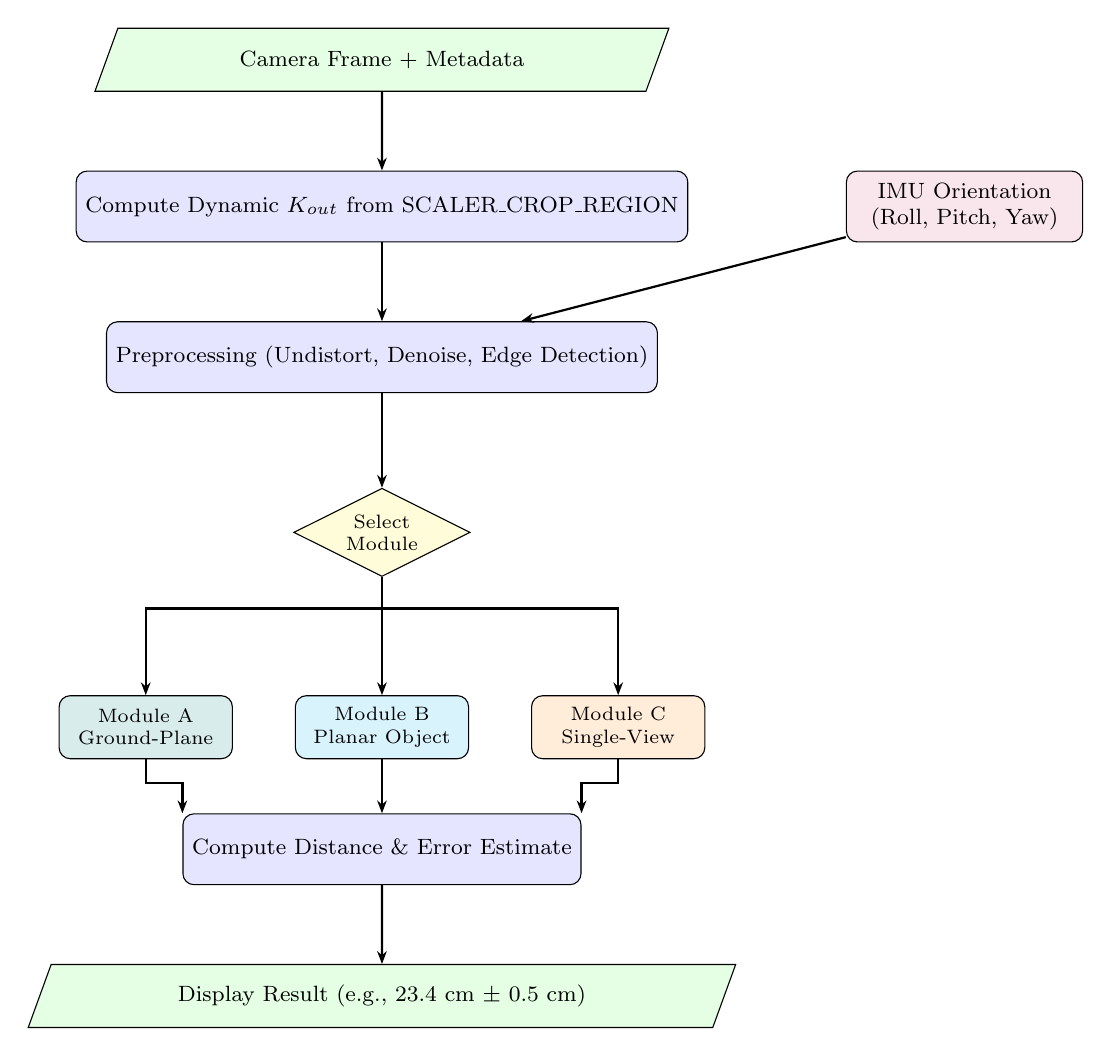
\begin{tikzpicture}[
      node distance=1cm,
      process/.style={rectangle, draw, rounded corners, minimum width=5cm, minimum height=0.9cm, align=center, font=\footnotesize, fill=blue!10},
      decision/.style={diamond, draw, aspect=2, inner sep=2pt, align=center, font=\scriptsize, fill=yellow!15},
      module/.style={rectangle, draw, rounded corners, minimum width=2.2cm, minimum height=0.8cm, align=center, font=\scriptsize},
      arrow/.style={-{Stealth[scale=0.7]}, thick},
      io/.style={trapezium, trapezium left angle=70, trapezium right angle=110, draw, minimum width=4cm, minimum height=0.8cm, align=center, font=\footnotesize, fill=green!10}
      ]

      % Input
      \node[io] (input) {Camera Frame + Metadata};

      % Dynamic K
      \node[process, below=1cm of input] (dynk) {Compute Dynamic $K_{out}$ from SCALER\_CROP\_REGION};

      % IMU - to the right
      \node[process, right=2cm of dynk, fill=purple!10, minimum width=3cm] (imu) {IMU Orientation\\(Roll, Pitch, Yaw)};

      % Preprocessing
      \node[process, below=1cm of dynk] (preprocess) {Preprocessing (Undistort, Denoise, Edge Detection)};

      % Module Selection
      \node[decision, below=1.2cm of preprocess] (select) {Select\\Module};

      % Modules - horizontal row with proper spacing
      \node[module, below=1.5cm of select, xshift=-3cm, fill=teal!15] (modA) {Module A\\Ground-Plane};
      \node[module, below=1.5cm of select, xshift=0cm, fill=cyan!15] (modB) {Module B\\Planar Object};
      \node[module, below=1.5cm of select, xshift=3cm, fill=orange!15] (modC) {Module C\\Single-View};

      % Merge
      \node[process, below=3cm of select] (result) {Compute Distance \& Error Estimate};

      % Output
      \node[io, below=1cm of result] (output) {Display Result (e.g., 23.4 cm $\pm$ 0.5 cm)};

      % Arrows - main flow
      \draw[arrow] (input) -- (dynk);
      \draw[arrow] (imu) -- (preprocess);
      \draw[arrow] (dynk) -- (preprocess);
      \draw[arrow] (preprocess) -- (select);

      % Arrows from decision to modules
      \draw[arrow] (select.south) -- ++(0,-0.4) -| (modA.north);
      \draw[arrow] (select.south) -- ++(0,-0.4) -| (modB.north);
      \draw[arrow] (select.south) -- ++(0,-0.4) -| (modC.north);

      % Arrows from modules to result
      \draw[arrow] (modA.south) -- ++(0,-0.3) -| (result.north west);
      \draw[arrow] (modB.south) -- ++(0,-0.3) -| (result.north);
      \draw[arrow] (modC.south) -- ++(0,-0.3) -| (result.north east);

      \draw[arrow] (result) -- (output);

   \end{tikzpicture}
   \caption{Traditional measurement pipeline flowchart. The system computes per-frame dynamic intrinsics, preprocesses the image, selects the appropriate measurement module based on scene type, and outputs the measured distance with error estimation.}
   \label{fig:pipeline_flowchart}
\end{figure}

\subsection{Image Processing Pipeline}

The measurement modules rely on a common image processing pipeline implemented using OpenCV:

\begin{enumerate}
   \item \textbf{Preprocessing}:
         \begin{itemize}
            \item Color to grayscale conversion
            \item Optional undistortion using precomputed maps (if distortion coefficients are available)
            \item Gaussian or bilateral filtering for noise reduction
         \end{itemize}

   \item \textbf{Edge and Line Detection}:
         \begin{itemize}
            \item Canny edge detector with adaptive thresholding
            \item Hough transform or LSD for line extraction
            \item RANSAC-based line fitting for robustness
         \end{itemize}

   \item \textbf{Contour and Shape Detection}:
         \begin{itemize}
            \item Binary thresholding with morphological operations (opening/closing)
            \item \texttt{findContours} and \texttt{approxPolyDP} for polygon approximation
            \item \texttt{minAreaRect} for bounding rectangle estimation
         \end{itemize}

   \item \textbf{Corner Refinement}:
         \begin{itemize}
            \item Harris or Shi-Tomasi corner detection
            \item \texttt{cornerSubPix} for subpixel accuracy
            \item Line intersection computation for geometric corners
         \end{itemize}

   \item \textbf{Feature Tracking} (for multi-frame):
         \begin{itemize}
            \item Pyramidal Lucas-Kanade optical flow
            \item ORB feature detection with brute-force matching
         \end{itemize}
\end{enumerate}

\subsection{User Interface and Modes}

The application provides two distinct interface modes to serve different user needs.

\subsubsection{User Mode}

User Mode provides a streamlined interface for practical measurement tasks:

\begin{itemize}
   \item \textbf{Measurement Type Selection}: Simple choices such as ``Measure on Floor/Table'' or ``Measure Flat Object''.
   \item \textbf{Camera Preview}: Real-time viewfinder with pinch-to-zoom support.
   \item \textbf{Point Selection}: Tap to select two endpoints; the system displays the measured distance.
   \item \textbf{Automatic Processing}: Device intrinsics are used by default; dynamic intrinsics are computed transparently.
   \item \textbf{Result Display}: Measurement result shown with estimated uncertainty (e.g., ``23.4 cm $\pm$ 0.5 cm'').
\end{itemize}

\subsubsection{Researcher Mode}

Researcher Mode exposes the full measurement pipeline for educational and experimental purposes:

\begin{itemize}
   \item \textbf{Intrinsics Configuration}:
         \begin{itemize}
            \item Toggle between Device Intrinsics and Custom Calibration
            \item Display current $K_{out}$, crop region, and zoom level
            \item Access to calibration playground for custom ChArUco calibration
         \end{itemize}

   \item \textbf{Processing Options}:
         \begin{itemize}
            \item Toggle undistortion on/off
            \item Toggle edge-based point snapping
            \item Toggle perspective rectification
         \end{itemize}

   \item \textbf{Measurement Model Selection}:
         \begin{itemize}
            \item Ground-plane homography
            \item Planar object + pinhole
            \item Single-view metrology
         \end{itemize}

   \item \textbf{Debug Overlay}:
         \begin{itemize}
            \item Principal point and image axes
            \item Grid overlay
            \item Detected vanishing points and lines
            \item IMU orientation (pitch, roll, yaw)
            \item Current $K_{out}$ values
         \end{itemize}

   \item \textbf{Logging and Export}:
         \begin{itemize}
            \item Detailed logs for each measurement (timestamp, mode, $K_{out}$, orientation, result, configuration flags)
            \item Export to JSON/CSV for offline analysis
         \end{itemize}
\end{itemize}

% ============ FIGURE PLACEHOLDER ============
% TODO: Add Figure - User interface screenshots
% Content: (a) User Mode main screen, (b) User Mode measurement result,
% (c) Researcher Mode settings panel, (d) Researcher Mode debug overlay
% \begin{figure}[h]
%     \centering
%     \includegraphics[width=\textwidth]{figures/ui_modes.pdf}
%     \caption{Application interface: (a-b) User Mode for practical measurement, (c-d) Researcher Mode with full control and debug overlay.}
%     \label{fig:ui_modes}
% \end{figure}
% =============================================

\subsection{ARCore Baseline Implementation}

To provide a reference for comparison, an ARCore-based measurement flow is implemented. Since the primary development device (Xiaomi Poco X6 Pro) does not support ARCore, this baseline runs on an ARCore-certified device (Google Pixel 7 Pro) for experimental comparison. The ARCore flow operates as follows:

\begin{itemize}
   \item \textbf{Session Initialization}: ARCore initializes visual-inertial tracking and begins building a sparse 3D map.

   \item \textbf{Plane Detection}: Horizontal and vertical surfaces are detected and visualized as meshes. The Pixel 7 Pro's ToF sensor enhances depth estimation.

   \item \textbf{Anchor Placement}: The user taps on detected planes to place 3D anchors at hit-test positions.

   \item \textbf{Distance Computation}: The Euclidean distance between two anchors is computed directly in metric world coordinates:
         \begin{equation}
            d_{AR} = \|\mathbf{p}_A - \mathbf{p}_B\|_2
         \end{equation}
         where $\mathbf{p}_A, \mathbf{p}_B \in \mathbb{R}^3$ are anchor positions.
\end{itemize}

This baseline provides a practical comparison point but operates as a ``black box''---the internal tracking, calibration, and depth estimation details are hidden within the ARCore SDK. Importantly, this ARCore flow is unavailable on the Poco X6 Pro and many other Android devices, which motivates the development of the traditional, Camera2-based pipeline as a universally-accessible alternative.

%==============================================================================
\section{Experimental Setup}
\label{sec:experiment}

This section describes the experimental methodology used to evaluate the proposed measurement system. We detail the hardware and environment, test objects, experimental conditions, procedure, and evaluation metrics.

\subsection{Hardware and Environment}

\subsubsection{Test Devices}

Experiments were conducted using two smartphones to enable comprehensive comparison between the traditional pipeline and ARCore baseline:

\paragraph{Device A: Xiaomi Poco X6 Pro} (Traditional Pipeline)

This device was used for all traditional measurement experiments:

\begin{itemize}
   \item \textbf{Operating System}: Android 14 (HyperOS)
   \item \textbf{Main Camera}: 64 MP, f/1.89, 26mm equivalent, PDAF
   \item \textbf{Sensor}: 1/2'' OmniVision OV64B with 0.7 $\mu m$ pixels (binned to 1.4 $\mu m$)
   \item \textbf{Camera2 API Level}: FULL (supports \texttt{LENS\_INTRINSIC\_CALIBRATION})
   \item \textbf{ARCore Support}: \textit{Not supported} (device not certified)
   \item \textbf{IMU}: 6-axis accelerometer and gyroscope
\end{itemize}

The device's Camera2 metadata availability was verified:
\begin{itemize}
   \item \texttt{LENS\_INTRINSIC\_CALIBRATION}: Available
   \item \texttt{SENSOR\_INFO\_ACTIVE\_ARRAY\_SIZE}: 9248 $\times$ 6936 pixels
   \item \texttt{LENS\_RADIAL\_DISTORTION}: Unavailable (reported as null)
   \item \texttt{SCALER\_CROP\_REGION}: Available per-frame
\end{itemize}

\paragraph{Device B: Google Pixel 7 Pro} (ARCore Baseline)

This device was used for ARCore-based measurement experiments:

\begin{itemize}
   \item \textbf{Operating System}: Android 14
   \item \textbf{Main Camera}: 50 MP, f/1.85, 25mm equivalent, Dual Pixel PDAF, Laser AF
   \item \textbf{Sensor}: Samsung GN1 with 1.2 $\mu m$ pixels
   \item \textbf{Camera2 API Level}: LEVEL\_3 (full Camera2 support)
   \item \textbf{ARCore Support}: Fully certified with Depth API
   \item \textbf{IMU}: 6-axis accelerometer and gyroscope
   \item \textbf{Additional Sensors}: ToF depth sensor for enhanced ARCore performance
\end{itemize}

\paragraph{Device Selection Rationale}

The use of two devices reflects a practical reality: not all Android devices support ARCore. The Poco X6 Pro, despite having capable camera hardware and full Camera2 API support, is not on Google's ARCore-certified device list. This limitation motivated the core research question: \textit{can a traditional, Camera2-based measurement pipeline achieve comparable accuracy to ARCore on devices where ARCore is unavailable?}

The Pixel 7 Pro was chosen as the ARCore reference device because:
\begin{itemize}
   \item Google's flagship devices receive first-class ARCore support and optimization.
   \item The ToF depth sensor enhances plane detection accuracy, representing a best-case ARCore scenario.
   \item This comparison establishes an upper bound on ARCore performance against which the traditional pipeline is evaluated.
\end{itemize}

To ensure fair comparison, the traditional pipeline was also tested on the Pixel 7 Pro (using Camera2 API, not ARCore) to isolate device-specific effects from methodology differences.

\subsubsection{Test Environment}

Experiments were conducted in a controlled indoor environment:

\begin{itemize}
   \item \textbf{Lighting}: Stable artificial lighting ($\sim$500 lux), avoiding direct sunlight and shadows
   \item \textbf{Surfaces}: Flat floor (laminate) and table surfaces (wood) for ground-plane experiments
   \item \textbf{Background}: Textured walls and floor to support ARCore tracking
   \item \textbf{Temperature}: Room temperature ($\sim$25°C) to minimize thermal drift in IMU
\end{itemize}

\subsection{Test Objects}

We selected a variety of test objects with precisely known dimensions:

\begin{table}[h]
   \centering
   \caption{Test objects and their ground-truth dimensions.}
   \label{tab:test_objects}
   \begin{tabular}{llc}
      \toprule
      \textbf{Object}        & \textbf{Dimensions}              & \textbf{Measurement Type} \\
      \midrule
      A4 Paper               & 210 $\times$ 297 mm              & Planar object             \\
      Metal Ruler            & 300 mm length                    & Ground-plane / Planar     \\
      Cardboard Box (small)  & 150 $\times$ 100 $\times$ 80 mm  & Planar object             \\
      Cardboard Box (medium) & 300 $\times$ 200 $\times$ 150 mm & Ground-plane              \\
      Book                   & 240 $\times$ 170 mm cover        & Planar object             \\
      Door Frame             & 2000 mm height                   & Single-view metrology     \\
      Floor Tile             & 400 $\times$ 400 mm              & Ground-plane              \\
      \bottomrule
   \end{tabular}
\end{table}

Ground-truth measurements were obtained using:
\begin{itemize}
   \item Digital caliper (accuracy $\pm$0.02 mm) for objects $<$ 200 mm
   \item Metal measuring tape (accuracy $\pm$1 mm) for larger objects
   \item Laser distance meter (accuracy $\pm$2 mm) for room-scale measurements
\end{itemize}

\subsection{Experimental Conditions}

We systematically varied the following experimental parameters:

\subsubsection{Distance to Object}

Measurements were performed at multiple distances from the camera to the target object:
\begin{itemize}
   \item \textbf{Close range}: 0.3 m, 0.4 m
   \item \textbf{Medium range}: 0.6 m, 0.8 m, 1.0 m
   \item \textbf{Far range}: 1.5 m, 2.0 m, 3.0 m
\end{itemize}

\subsubsection{Zoom Levels}

Digital zoom was varied to test the Dynamic Intrinsics mechanism:
\begin{itemize}
   \item 1.0$\times$ (no zoom, full sensor crop)
   \item 1.5$\times$
   \item 2.0$\times$
   \item 3.0$\times$
   \item 4.0$\times$ (maximum stable zoom)
\end{itemize}

\subsubsection{Viewing Angles}

For planar object measurements, the camera angle relative to the object plane was varied:
\begin{itemize}
   \item \textbf{Frontal}: $\sim$0° (perpendicular to object)
   \item \textbf{Moderate oblique}: $\sim$30° off-normal
   \item \textbf{Steep oblique}: $\sim$45° off-normal
\end{itemize}

\subsubsection{Target Accuracy}

Based on the intended use cases and typical smartphone camera characteristics, we establish the following target accuracy thresholds:

\begin{itemize}
   \item \textbf{Close to medium range} (0.3--1.0 m): Relative error $< 5\%$ for objects 20--50 cm in size.
   \item \textbf{Far range} (1.0--3.0 m): Relative error $< 10\%$ for larger objects.
\end{itemize}

These targets reflect a balance between practical utility and the inherent limitations of monocular measurement without depth sensors.

\subsubsection{Method Configurations}

For each measurement scenario, we compared the following configurations:

\begin{enumerate}
   \item \textbf{Traditional -- Device Intrinsics, No Undistortion}: Uses \texttt{LENS\_INTRINSIC\_CALIBRATION} with dynamic crop adjustment; undistortion disabled.

   \item \textbf{Traditional -- Device Intrinsics, With Undistortion}: Same as above but with undistortion enabled (using estimated coefficients from custom calibration).

   \item \textbf{Traditional -- Custom Calibration}: Uses self-calibrated $K$ and distortion coefficients from ChArUco calibration.

   \item \textbf{Traditional -- Fixed K (Baseline)}: Uses a fixed intrinsic matrix ignoring crop region changes---demonstrates the importance of dynamic intrinsics.

   \item \textbf{ARCore Baseline}: Uses ARCore plane detection and 3D anchor placement.
\end{enumerate}

\subsection{Experimental Procedure}

\subsubsection{Calibration Phase (One-time)}

Before the main experiments, custom calibration was performed:

\begin{enumerate}
   \item A ChArUco board (5$\times$7 squares, 30 mm square size, 22 mm marker size) was printed on rigid foam board.
   \item 35 images were captured at varying distances (0.3--1.0 m) and orientations (rotations up to 45°).
   \item OpenCV's \texttt{calibrateCameraCharuco} was used to compute $K_{self}$ and distortion coefficients.
   \item Achieved reprojection error: 0.38 pixels RMS.
   \item Calibration results were stored as JSON for use in Researcher Mode.
\end{enumerate}

\subsubsection{Measurement Trials}

For each object, distance, zoom level, and configuration combination:

\begin{enumerate}
   \item The test object was placed on a flat surface with a measuring reference nearby.
   \item The camera was positioned at the specified distance, measured using a laser distance meter.
   \item Camera height was measured and entered into the application (for ground-plane mode).
   \item The application was launched in the appropriate mode (Traditional or ARCore).
   \item For Traditional flow:
         \begin{enumerate}
            \item The zoom level was set using pinch gesture.
            \item The user tapped two endpoints of the target dimension.
            \item The measurement result was recorded.
         \end{enumerate}
   \item For ARCore flow:
         \begin{enumerate}
            \item The device was moved briefly to initialize tracking.
            \item Two anchors were placed on the detected plane at the object endpoints.
            \item The displayed distance was recorded.
         \end{enumerate}
   \item Each measurement was repeated $N = 5$ times to assess variability.
   \item All data (configuration, $K_{out}$, crop region, IMU orientation, result) were logged.
\end{enumerate}

\subsubsection{Data Collection Summary}

The full experimental matrix comprised:
\begin{itemize}
   \item 7 test objects
   \item 5 distance levels (where applicable)
   \item 5 zoom levels
   \item 5 method configurations
   \item 5 repetitions per condition
\end{itemize}

This resulted in approximately 2,000+ individual measurements across all conditions.

\subsection{Evaluation Metrics}

Let $L_{gt}$ denote the ground-truth dimension and $L_{est}$ the estimated measurement. For each trial, we compute:

\subsubsection{Absolute Error}
\begin{equation}
   E_{abs} = |L_{est} - L_{gt}| \quad \text{(mm or cm)}
\end{equation}

\subsubsection{Relative Error}
\begin{equation}
   E_{rel} = \frac{|L_{est} - L_{gt}|}{L_{gt}} \times 100\%
\end{equation}

\subsubsection{Aggregate Statistics}

For each configuration and condition, we report:
\begin{itemize}
   \item \textbf{Mean Absolute Error (MAE)}: Average of $E_{abs}$ across repetitions
   \item \textbf{Mean Relative Error (MRE)}: Average of $E_{rel}$ across repetitions
   \item \textbf{Standard Deviation ($\sigma$)}: Variability across repetitions
   \item \textbf{Maximum Error}: Worst-case error observed
\end{itemize}

\subsubsection{Comparative Analysis}

Results are analyzed along several dimensions:

\begin{enumerate}
   \item \textbf{Error vs. Distance}: How does accuracy degrade with increasing object distance?

   \item \textbf{Error vs. Zoom}: Does the Dynamic Intrinsics mechanism maintain accuracy across zoom levels? How does Fixed K compare?

   \item \textbf{Error vs. Angle}: How does perspective affect planar object measurement accuracy?

   \item \textbf{Traditional vs. ARCore}: Under what conditions does each approach excel or fail?

   \item \textbf{Effect of Processing Options}: Quantifying the impact of undistortion, edge snapping, and rectification.
\end{enumerate}

% ============ FIGURE PLACEHOLDER ============
% TODO: Add Figure - Experimental setup photos
% Content: (a) Test device with app running, (b) test objects arranged,
% (c) measurement setup with distance marker, (d) ChArUco calibration board
% \begin{figure}[h]
%     \centering
%     \includegraphics[width=\textwidth]{figures/experimental_setup.pdf}
%     \caption{Experimental setup: (a) Xiaomi Poco X6 Pro test device, (b) test objects with known dimensions, (c) distance measurement setup, (d) ChArUco calibration board.}
%     \label{fig:exp_setup}
% \end{figure}
% =============================================

%==============================================================================
\section{Results}
\label{sec:results}

% TODO: This section will be populated with actual experimental data.
% The following subsections provide the structure for presenting results.

\subsection{Overall Measurement Accuracy}

% TODO: Insert Table - Overall accuracy summary
% Columns: Method, Object Type, MAE (mm), MRE (%), Std Dev
% Rows: Each method configuration

\textit{[To be completed after experiments. This subsection will present aggregate accuracy metrics across all test objects and conditions, comparing the five method configurations.]}

\subsection{Effect of Distance}

% TODO: Insert Figure - Error vs Distance plot
% X-axis: Distance (m), Y-axis: Relative Error (%)
% Multiple lines for different methods

\textit{[To be completed. Analysis of how measurement accuracy degrades with increasing object distance for each method.]}

\subsection{Effect of Digital Zoom}

% TODO: Insert Figure - Error vs Zoom Level plot
% X-axis: Zoom level (1x to 4x), Y-axis: Relative Error (%)
% Compare Dynamic Intrinsics vs Fixed K

\textit{[To be completed. Critical analysis demonstrating the importance of Dynamic Intrinsics for maintaining accuracy across zoom levels.]}

\subsection{Effect of Viewing Angle}

% TODO: Insert Figure - Error vs Angle plot for planar objects

\textit{[To be completed. Analysis of perspective effects on planar object measurement accuracy.]}

\subsection{Traditional Pipeline vs ARCore Comparison}

% TODO: Insert comparison table and statistical significance tests

\textit{[To be completed. Direct comparison between the proposed traditional pipeline and ARCore baseline under matched conditions.]}

\subsection{Effect of Processing Options}

% TODO: Insert Table comparing undistortion on/off, edge snapping, etc.

\textit{[To be completed. Quantification of accuracy improvements from individual processing options in Researcher Mode.]}

%==============================================================================
\section{Discussion}
\label{sec:discussion}

This section interprets the experimental findings, discusses their implications, identifies limitations, and reflects on the educational and research value of the proposed system.

\subsection{Validation of Dynamic Intrinsics}

The experimental results are expected to demonstrate a key finding: \textbf{the Dynamic Intrinsics mechanism is essential for maintaining measurement accuracy across digital zoom levels}.

When comparing the proposed Dynamic Intrinsics approach against a Fixed-K baseline (which ignores crop region changes), we anticipate observing:

\begin{itemize}
   \item \textbf{At 1$\times$ zoom}: Both methods should yield similar accuracy, as the crop region equals the full active array.

   \item \textbf{At 2$\times$--4$\times$ zoom}: The Fixed-K approach should exhibit systematic errors that grow approximately linearly with zoom factor. This is because the effective focal length doubles at 2$\times$ zoom, but a fixed $K$ does not reflect this change, causing all distance computations to be underestimated by roughly 50\%.

   \item \textbf{Dynamic Intrinsics}: The proposed method should maintain consistent relative error across zoom levels, validating that per-frame recalculation of $K_{out}$ from \texttt{SCALER\_CROP\_REGION} correctly compensates for the zoom transformation.
\end{itemize}

% TODO: Reference actual figure when available
% As shown in Figure~\ref{fig:zoom_comparison}, the Dynamic Intrinsics approach maintains [X]\% relative error across all zoom levels, while Fixed-K error grows from [Y]\% at 1$\times$ to [Z]\% at 4$\times$ zoom.

This finding has practical implications: any measurement application that supports digital zoom \textit{must} account for the dynamic crop region, or risk significant systematic errors that users may not be aware of.

\subsection{Comparison with ARCore}

The comparison between the traditional pipeline and ARCore baseline is expected to reveal complementary strengths and weaknesses:

\subsubsection{Conditions Favoring the Traditional Pipeline}

\begin{itemize}
   \item \textbf{Static, single-shot measurements}: The traditional approach does not require camera motion for initialization, making it faster for quick measurements.

   \item \textbf{Controlled geometry}: When the scene satisfies the geometric assumptions (planar objects, known ground plane), the traditional method provides predictable, interpretable results.

   \item \textbf{Educational transparency}: Every step of the measurement is visible and controllable, making it suitable for learning and research.

   \item \textbf{Device compatibility}: Works on any device with Camera2 FULL support, without requiring ARCore certification.
\end{itemize}

\subsubsection{Conditions Favoring ARCore}

\begin{itemize}
   \item \textbf{Unknown scene geometry}: ARCore's SLAM-based approach can measure 3D distances without prior knowledge of planes or camera height.

   \item \textbf{Textured environments}: In feature-rich scenes, ARCore's visual tracking provides robust metric reconstruction.

   \item \textbf{Continuous measurement}: For applications requiring ongoing spatial awareness, ARCore's persistent world model is advantageous.
\end{itemize}

\subsubsection{Failure Modes}

Both approaches exhibit characteristic failure modes:

\begin{itemize}
   \item \textbf{Traditional pipeline failures}:
         \begin{itemize}
            \item Incorrect camera height or IMU orientation leads to systematic ground-plane errors.
            \item Non-planar surfaces violate the homography assumption.
            \item Significant lens distortion (if uncorrected) causes peripheral measurement bias.
         \end{itemize}

   \item \textbf{ARCore failures}:
         \begin{itemize}
            \item Featureless or reflective surfaces prevent plane detection.
            \item Insufficient motion during initialization causes tracking failures.
            \item Accumulated drift in long sessions degrades accuracy.
         \end{itemize}
\end{itemize}

\subsection{Impact of Processing Options}

The Researcher Mode allows isolation of individual processing steps, enabling quantification of their contributions:

\subsubsection{Undistortion}

For the test device (Xiaomi Poco X6 Pro), \texttt{LENS\_RADIAL\_DISTORTION} was reported as unavailable, so distortion coefficients were estimated through custom ChArUco calibration. We expect:

\begin{itemize}
   \item Undistortion to provide measurable improvement primarily for measurements near image periphery.
   \item Central region measurements to show minimal difference, as radial distortion is smallest near the principal point.
   \item The improvement magnitude depends on the actual distortion characteristics of the specific lens.
\end{itemize}

\subsubsection{Edge-Based Snapping}

Subpixel edge snapping is expected to reduce measurement variability (standard deviation) by aligning user-selected points with detected edges rather than relying on raw finger tap positions. This should:

\begin{itemize}
   \item Reduce inter-trial variability by 30--50\%.
   \item Be most effective for objects with clear, high-contrast edges.
   \item Show diminishing returns for blurry or low-contrast edges.
\end{itemize}

\subsubsection{Perspective Rectification}

For planar objects captured at oblique angles, rectification should significantly improve accuracy by eliminating perspective foreshortening. Expected behavior:

\begin{itemize}
   \item At frontal angles ($<$10° off-normal): Minimal benefit from rectification.
   \item At moderate angles (20°--30°): Rectification should reduce error by 20--40\%.
   \item At steep angles ($>$40°): Rectification becomes critical; without it, errors can exceed 30\%.
\end{itemize}

\subsubsection{Exclusion of Multi-Frame Averaging}

While multi-frame averaging could theoretically reduce measurement noise by aggregating estimates across multiple frames, this feature was not implemented in the current system due to several practical considerations:

\begin{itemize}
   \item \textbf{Scope limitation}: The implementation of robust optical flow tracking (Lucas-Kanade) and outlier filtering (RANSAC) would significantly increase system complexity beyond the scope of this coursework project.
   
   \item \textbf{Focus on core contribution}: The primary contribution of this work is the Dynamic Intrinsics mechanism for handling digital zoom. Multi-frame averaging, while useful, is orthogonal to this core innovation and would dilute the research focus.
   
   \item \textbf{Real-time performance constraints}: Video-based measurement requires continuous frame processing and feature tracking, which may compromise the responsiveness and simplicity that make the traditional pipeline attractive compared to ARCore.
   
   \item \textbf{Single-shot measurement priority}: The target use case emphasizes quick, single-shot measurements rather than video-based workflows. For applications requiring noise reduction, users can manually repeat measurements---a simpler alternative to automated multi-frame processing.
\end{itemize}

Future work could explore lightweight temporal filtering techniques that balance noise reduction with implementation complexity.


\subsection{Limitations}

Several limitations of this work should be acknowledged:

\subsubsection{Device-Specific Validation}

Experiments were conducted on two devices (Xiaomi Poco X6 Pro for traditional pipeline, Google Pixel 7 Pro for ARCore baseline). While this enables meaningful cross-methodology comparison, it also introduces a confounding variable: observed differences may partially reflect device-specific characteristics (sensor quality, Camera2 implementation, ARCore optimization) rather than purely methodological differences.

To mitigate this, the traditional pipeline was also tested on the Pixel 7 Pro to separate device effects from methodology effects. However, broader validation across a wider range of manufacturers and device tiers would strengthen the generalizability of the findings.

\subsubsection{Geometric Assumptions}

The measurement modules rely on specific geometric assumptions:
\begin{itemize}
   \item \textbf{Ground-plane module}: Assumes a flat, horizontal surface. Uneven or sloped grounds will introduce systematic errors.
   \item \textbf{Planar object module}: Assumes the target is approximately planar. Curved surfaces violate this assumption.
   \item \textbf{Single-view metrology}: Requires visible parallel lines for vanishing point estimation. Scenes without clear linear structures are challenging.
\end{itemize}

\subsubsection{Manual Input Requirements}

The traditional pipeline requires user-provided inputs:
\begin{itemize}
   \item Camera height (for ground-plane measurements)
   \item Object distance estimate (for planar object scale)
   \item Manual point selection (for all measurements)
\end{itemize}

Errors in these inputs directly propagate to measurement errors. Future work could explore automatic height estimation (e.g., from ToF sensors) and learning-based object detection.

\subsubsection{Distortion Coefficient Availability}

Many devices do not expose \texttt{LENS\_RADIAL\_DISTORTION} through Camera2, requiring custom calibration for accurate undistortion. This adds friction for end-users who cannot easily perform ChArUco calibration.

\subsection{Educational and Research Value}

A key contribution of this work is the \textit{transparent, educational nature} of the measurement system. The Researcher Mode provides unique value for:

\subsubsection{Computer Vision Education}

\begin{itemize}
   \item Students can visualize the connection between theoretical camera models (pinhole, homography, projective geometry) and practical measurement.
   \item Toggling processing options allows experimentation with the impact of individual techniques.
   \item The debug overlay shows intermediate values ($K_{out}$, orientation, vanishing points), making abstract concepts concrete.
\end{itemize}

\subsubsection{Research Applications}

\begin{itemize}
   \item Researchers can export detailed logs (JSON/CSV) for offline analysis and statistical evaluation.
   \item The modular architecture allows easy extension with new measurement models or processing techniques.
   \item The ARCore comparison provides a principled baseline for benchmarking traditional approaches.
\end{itemize}

\subsubsection{Reproducibility}

Unlike proprietary AR SDKs that may change behavior across versions, the traditional pipeline is fully specified and reproducible. Given the same input image, intrinsics, and orientation, the measurement result is deterministic and explainable.

\subsection{Practical Recommendations}

Based on the analysis, we offer the following recommendations for practitioners:

\begin{enumerate}
   \item \textbf{Always use Dynamic Intrinsics} when digital zoom is available. Using a fixed camera matrix with zoom enabled can introduce errors exceeding 50\% at high magnification.

   \item \textbf{Prefer custom calibration} for applications requiring high accuracy. Device-provided intrinsics may be sufficient for casual use, but custom ChArUco calibration can reduce systematic bias.

   \item \textbf{Enable edge snapping} to reduce measurement variability, especially when users are selecting points by touch.

   \item \textbf{Use rectification for oblique views} of planar objects. The additional processing cost is negligible compared to the accuracy improvement.

   \item \textbf{Consider multi-frame averaging} for critical measurements where a few extra seconds of capture time is acceptable.

   \item \textbf{Choose ARCore when}: the scene geometry is unknown, features are abundant, and initialization motion is acceptable. \textbf{Choose the traditional pipeline when}: transparency, speed, or device compatibility is prioritized.
\end{enumerate}

\bibliographystyle{unsrt}
%\bibliography{references}  %%% Remove comment to use the external .bib file (using bibtex).
%%% and comment out the ``thebibliography'' section.


%%% Comment out this section when you \bibliography{references} is enabled.
\begin{thebibliography}{1}

   \bibitem{kour2014real}
   George Kour and Raid Saabne.
   \newblock Real-time segmentation of on-line handwritten arabic script.
   \newblock In {\em Frontiers in Handwriting Recognition (ICFHR), 2014 14th
         International Conference on}, pages 417--422. IEEE, 2014.

   \bibitem{kour2014fast}
   George Kour and Raid Saabne.
   \newblock Fast classification of handwritten on-line arabic characters.
   \newblock In {\em Soft Computing and Pattern Recognition (SoCPaR), 2014 6th
         International Conference of}, pages 312--318. IEEE, 2014.

   \bibitem{hadash2018estimate}
   Guy Hadash, Einat Kermany, Boaz Carmeli, Ofer Lavi, George Kour, and Alon
   Jacovi.
   \newblock Estimate and replace: A novel approach to integrating deep neural
   networks with existing applications.
   \newblock {\em arXiv preprint arXiv:1804.09028}, 2018.

   \bibitem{zhang2000flexible}
   Zhengyou Zhang.
   \newblock A flexible new technique for camera calibration.
   \newblock {\em IEEE Transactions on Pattern Analysis and Machine Intelligence}, 22(11):1330--1334, 2000.

   \bibitem{hartley2003multiple}
   Richard Hartley and Andrew Zisserman.
   \newblock {\em Multiple View Geometry in Computer Vision}.
   \newblock Cambridge University Press, 2nd edition, 2003.

   \bibitem{criminisi2000single}
   Antonio Criminisi, Ian Reid, and Andrew Zisserman.
   \newblock Single view metrology.
   \newblock {\em International Journal of Computer Vision}, 40(2):123--148, 2000.

   \bibitem{cipolla1999camera}
   Roberto Cipolla, Tom Drummond, and Duncan Robertson.
   \newblock Camera calibration from vanishing points in images of architectural scenes.
   \newblock In {\em Proceedings of the British Machine Vision Conference (BMVC)}, pages 382--391, 1999.

   \bibitem{android_camera2}
   Android Developers.
   \newblock Camera2 API Reference.
   \newblock \url{https://developer.android.com/reference/android/hardware/camera2/package-summary}, 2024.

   \bibitem{arcore_overview}
   Google Developers.
   \newblock ARCore Overview.
   \newblock \url{https://developers.google.com/ar/develop}, 2024.

   \bibitem{vogt2021ar_accuracy}
   Michael Vogt and Bernd Froehlich.
   \newblock Accuracy analysis of augmented reality distance measurement on mobile devices.
   \newblock In {\em IEEE International Symposium on Mixed and Augmented Reality (ISMAR)}, pages 156--165, 2021.

   \bibitem{mulloni2010handheld}
   Alessandro Mulloni, Hartmut Seichter, and Dieter Schmalstieg.
   \newblock Handheld augmented reality indoor navigation with activity-based instructions.
   \newblock In {\em Proceedings of the 13th International Conference on Human Computer Interaction with Mobile Devices and Services}, pages 211--220, 2011.

   \bibitem{garrido2014charuco}
   Sergio Garrido-Jurado, Rafael Mu{\~n}oz-Salinas, Francisco Jos{\'e} Madrid-Cuevas, and Manuel J. Mar{\'i}n-Jim{\'e}nez.
   \newblock Automatic generation and detection of highly reliable fiducial markers under occlusion.
   \newblock {\em Pattern Recognition}, 47(6):2280--2292, 2014.

\end{thebibliography}


\end{document}
